% !TeX program = xelatex
% !TeX encoding = utf-8
\documentclass[aspectratio=169, 11pt]{beamer}

% ==============================================================================
% Cấu hình Font và Ngôn ngữ (Segoe UI & Consolas)
% ==============================================================================
\usepackage{fontspec}
\defaultfontfeatures{Ligatures=TeX}
\setsansfont{Segoe UI}[
  BoldFont = {Segoe UI Bold},
  ItalicFont = {Segoe UI Italic},
  BoldItalicFont = {Segoe UI Bold Italic}
]
\setmonofont[Scale=0.90]{Consolas}[
  BoldFont = {Consolas Bold},
  ItalicFont = {Consolas Italic},
  BoldItalicFont = {Consolas Bold Italic}
]

\usepackage{amsmath,amssymb}
\usepackage{booktabs}
\usepackage{array}
\usepackage{tabularx}
\usepackage{colortbl}
\usepackage{graphicx}
\usepackage{xcolor}
\usepackage{fancyvrb}
\usepackage[many]{tcolorbox}
\usepackage{tikz}
\usetikzlibrary{arrows.meta, positioning, calc, patterns, shapes.geometric}

\graphicspath{{figures/}{./}}

% ==============================================================================
% Bảng màu chuẩn Khoa Điện tử (ĐHBK - ĐHĐN)
% ==============================================================================
\definecolor{FacultyNavy}{RGB}{0, 0, 76}        % Xanh Navy chuẩn slide Khoa (#00004C)
\definecolor{FacultyYellow}{RGB}{255, 191, 0}    % Vàng chuẩn slide Khoa (#FFBF00)
\definecolor{DarkMain}{RGB}{20, 20, 20}         % Màu đen viền khung & tiêu đề (#141414)
\definecolor{NavyDark}{RGB}{0, 0, 76}           % Đồng bộ Navy chuẩn
\definecolor{TealAccent}{RGB}{255, 191, 0}      % Điểm nhấn vàng chuẩn
\definecolor{BoxMain}{RGB}{225, 228, 233}       % Màu khối sơ đồ TikZ
\definecolor{BoxSub}{RGB}{246, 247, 249}        % Màu khối sơ đồ phụ
\definecolor{CodeBg}{RGB}{247, 248, 250}        % Màu nền khối mã nguồn
\definecolor{TextDark}{RGB}{20, 20, 20}         % Màu chữ nội dung
\definecolor{TextMuted}{RGB}{100, 102, 108}     % Màu chú thích / thứ cấp

% ==============================================================================
% Cấu hình giao diện Beamer
% ==============================================================================
\useinnertheme{default}
\useoutertheme{default}
\setbeamertemplate{navigation symbols}{}
\setbeamersize{text margin left=0.85cm, text margin right=0.85cm}

\setbeamertemplate{footline}{}
\newcommand{\setsectionfooter}[1]{}

\setbeamercolor{background canvas}{bg=white}
\setbeamercolor{normal text}{fg=TextDark}
\setbeamercolor{itemize item}{fg=DarkMain}
\setbeamercolor{itemize subitem}{fg=TextMuted}

% Định dạng dấu đầu dòng hình vuông đen chuẩn slide Khoa
\setbeamertemplate{itemize item}{\raisebox{0.14ex}{\color{DarkMain}\rule{1.0ex}{1.0ex}}}
\setbeamertemplate{itemize subitem}{\raisebox{0.18ex}{\color{TextMuted}\rule{0.8ex}{0.8ex}}}
\setbeamertemplate{enumerate item}{\textbf{\color{DarkMain}\insertenumlabel.}}

% ==============================================================================
% Header Widget chuẩn Khoa Điện tử (ĐHBK ĐHĐN)
% ==============================================================================
\setbeamertemplate{frametitle}{%
  \begin{tikzpicture}[remember picture, overlay]
    % 1. Logo Khoa & Tên Khoa
    \node[anchor=west, inner sep=0pt] at ([shift={(0.30cm, -0.53cm)}]current page.north west) {
      
\includegraphics[height=0.68cm, keepaspectratio]{figures/logo_khoa.jpg}
    };
    \node[anchor=west, inner sep=0pt] at ([shift={(1.08cm, -0.53cm)}]current page.north west) {
      \begin{minipage}{2.35cm}
        \fontsize{5.2pt}{6.2pt}\selectfont\bfseries\color{FacultyNavy}
        KHOA ĐIỆN TỬ VÀ\\[1.0pt]
        TRÍ TUỆ NHÂN TẠO
      \end{minipage}
    };

    % 2. Dải xiên màu vàng
    \fill[FacultyYellow] 
      ([shift={(3.75cm, 0)}]current page.north west) -- 
      ([shift={(4.35cm, 0)}]current page.north west) -- 
      ([shift={(3.90cm, -1.06cm)}]current page.north west) -- 
      ([shift={(3.30cm, -1.06cm)}]current page.north west) -- cycle;
      
    % 3. Khối chữ nhật vát xanh Navy
    \fill[FacultyNavy] 
      ([shift={(4.35cm, 0)}]current page.north west) -- 
      (current page.north east) -- 
      ([shift={(0, -1.06cm)}]current page.north east) -- 
      ([shift={(3.90cm, -1.06cm)}]current page.north west) -- cycle;
      
    % 4. Tiêu đề slide
    \node[anchor=west, text=white, font=\fontsize{11.2pt}{13.2pt}\selectfont\bfseries, text width=10.2cm, align=left] 
      at ([shift={(4.60cm, -0.53cm)}]current page.north west) {
      \insertframetitle
    };
    
    % 5. Số trang màu vàng 2 chữ số nổi bật
    \node[anchor=east, text=FacultyYellow, font=\fontsize{14pt}{16pt}\selectfont\bfseries] 
      at ([shift={(-0.45cm, -0.53cm)}]current page.north east) {
      \ifnum\insertframenumber<10 0\fi\insertframenumber
    };
  \end{tikzpicture}%
  \vspace{0.40cm}%
}

% ==============================================================================
% Định dạng các khối Card và Sơ đồ TikZ
% ==============================================================================
\newcommand{\code}[1]{\leavevmode{\ttfamily\color{DarkMain}#1}}

\tikzset{
  >=Stealth,
  diagbox/.style={
    rectangle,
    rounded corners=2.2pt,
    draw=DarkMain,
    line width=0.9pt,
    fill=BoxMain,
    minimum height=0.75cm,
    align=center,
    font=\small\bfseries,
    text=TextDark
  },
  subbox/.style={
    rectangle,
    rounded corners=2.2pt,
    draw=DarkMain,
    line width=0.9pt,
    fill=BoxSub,
    minimum height=0.75cm,
    align=center,
    font=\small,
    text=TextDark
  },
  flowarrow/.style={
    -{Stealth[length=2.3mm, width=1.7mm]},
    draw=DarkMain,
    line width=0.95pt
  }
}

% ==============================================================================
% BẮT ĐẦU TÀI LIỆU
% ==============================================================================
\begin{document}

% ------------------------------------------------------------------------------
% SLIDE 1: TIÊU ĐỀ THEO CHUẨN NHẬN DIỆN THƯƠNG HIỆU KHOA
% ------------------------------------------------------------------------------
\begin{frame}[plain]
  \begin{tikzpicture}[remember picture, overlay]
    % 1. Nền trắng toàn trang
    \fill[white] (current page.south west) rectangle (current page.north east);

    % 2. Khối Dark Navy chính
    \fill[FacultyNavy] 
      (current page.north west) --
      ([shift={(10.4cm, 0)}]current page.north west) --
      ([shift={(0, -5.6cm)}]current page.north east) --
      (current page.south east) --
      ([shift={(2.1cm, 0)}]current page.south west) --
      ([shift={(0, 2.1cm)}]current page.south west) --
      cycle;

    % 3. Dải vàng góc trên-phải
    \fill[FacultyYellow]
      ([shift={(10.5cm, 0)}]current page.north west) --
      ([shift={(11.0cm, 0)}]current page.north west) --
      ([shift={(0, -5.0cm)}]current page.north east) --
      ([shift={(0, -5.5cm)}]current page.north east) --
      cycle;

    % 4. Dải vàng góc dưới-trái
    \fill[FacultyYellow]
      ([shift={(0, 1.5cm)}]current page.south west) --
      ([shift={(0, 2.0cm)}]current page.south west) --
      ([shift={(2.0cm, 0)}]current page.south west) --
      ([shift={(1.5cm, 0)}]current page.south west) --
      cycle;

    % 5. Circular badge ở góc trên phải
    \node[anchor=center] at ([shift={(13.25cm, -2.50cm)}]current page.north west) {
      
\includegraphics[width=2.50cm, height=2.50cm, keepaspectratio]{figures/badge_circle_alpha.png}
    };

    % 6. Tên Khoa ở góc trên trái
    \node[anchor=north west, text=white, font=\fontsize{11.5pt}{15pt}\selectfont\bfseries] 
      at ([shift={(1.0cm, -0.95cm)}]current page.north west) {
      KHOA ĐIỆN TỬ VÀ TRÍ TUỆ NHÂN TẠO
    };

    % 7. Tiêu đề báo cáo tiến độ
    \node[anchor=north west, text=white!95, font=\fontsize{10.0pt}{13.0pt}\selectfont\bfseries] 
      at ([shift={(1.0cm, -2.15cm)}]current page.north west) {
      BÁO CÁO TIẾN ĐỘ LẦN 2 --- HỌC PHẦN: CÔNG NGHỆ PHẦN MỀM
    };

    % 8. Đường line phân cách màu vàng
    \draw[FacultyYellow!70, line width=1.1pt] 
      ([shift={(1.0cm, -2.75cm)}]current page.north west) -- ([shift={(10.8cm, -2.75cm)}]current page.north west);

    % 9. Tên đề tài chính
    \node[anchor=north west, text=FacultyYellow, font=\fontsize{15.0pt}{20.5pt}\selectfont\bfseries, text width=10.5cm] 
      at ([shift={(1.0cm, -3.30cm)}]current page.north west) {
      HỆ THỐNG GIÁM SÁT GIAO THÔNG VÀ CẢNH BÁO VA CHẠM DỰA TRÊN DUNG HỢP RADAR VÀ CAMERA
    };

    % 10. Thông tin Giảng viên & Sinh viên
    \node[anchor=north west, text=white, font=\fontsize{8.5pt}{12.2pt}\selectfont] 
      at ([shift={(3.8cm, -5.35cm)}]current page.north west) {
      \renewcommand{\arraystretch}{1.16}
      \begin{tabular}{@{}ll@{}}
        \textbf{Giảng viên hướng dẫn:} & TS. Đào Duy Tuấn \\[2.2pt]
        \textbf{Sinh viên thực hiện:}   & Ngô Quang Thế \quad (MSSV: 106230028 --- Nhóm trưởng) \\
                                        & Lê Anh Khoa \quad (MSSV: 106230016) \\
                                        & Huỳnh Ngọc Tịnh Phong \quad (MSSV: 106230022) \\[2.2pt]
        \textbf{Lớp sinh hoạt:}        & 23KTMT1 \quad\textbar\quad Nhóm 5
      \end{tabular}
    };

    % 11. Địa điểm & Năm
    \node[anchor=south, text=white!60, font=\fontsize{7.8pt}{10pt}\selectfont] 
      at ([shift={(1.0cm, 0.32cm)}]current page.south) {
      ĐÀ NẴNG, 2026
    };
  \end{tikzpicture}
\end{frame}

% ------------------------------------------------------------------------------
% SLIDE 2: PHÂN CÔNG NHIỆM VỤ & TRÁCH NHIỆM THÀNH VIÊN
% ------------------------------------------------------------------------------
\begin{frame}{Phân công Nhiệm vụ Thành viên}
  \vspace{0.15cm}

  \renewcommand{\arraystretch}{1.42}
  \fontsize{8.2pt}{10.8pt}\selectfont
  \centering
  \begin{tabularx}{\textwidth}{@{} p{3.4cm} p{3.1cm} X c @{}}
    \toprule[1.0pt]
    \textbf{Thành viên} & \textbf{Mảng phụ trách} & \textbf{Công việc kỹ thuật đã hoàn thành trong Giai đoạn 2} & \textbf{Tiến độ} \\
    \midrule[0.6pt]
    \textbf{Ngô Quang Thế}\newline{\fontsize{7.4pt}{9.0pt}\selectfont\color{TextMuted}(34\% --- \textit{Nhóm trưởng})} &
    Kiến trúc Hệ thống\newline\& Module CSDL Kép &
    Tích hợp CSDL mạng MySQL tập trung qua XAMPP, cơ chế tự động Failover sang SQLite; lập trình phân quyền dữ liệu theo tài khoản; đóng gói file \code{.exe}. &
    \textbf{95\%} \\
    \midrule[0.3pt]

    \textbf{Lê Anh Khoa}\newline{\fontsize{7.4pt}{9.0pt}\selectfont\color{TextMuted}(33\%)} &
    Giao diện PyQt6\newline\& Radar Canvas 2D &
    Tối ưu hóa giao diện đa độ phân giải (1366$\times$768 \& 1920$\times$1080); bản đồ Radar 2D QPainter thời gian thực; tích hợp đèn báo trạng thái CSDL trên Header. &
    \textbf{95\%} \\
    \midrule[0.3pt]

    \textbf{Huỳnh Ngọc Tịnh Phong}\newline{\fontsize{7.4pt}{9.0pt}\selectfont\color{TextMuted}(33\%)} &
    Thị giác máy tính AI\newline\& Phần cứng Cảm biến &
    Tối ưu nhận diện YOLOv8n ONNX trên luồng nền; kết nối và đo kiểm cảm biến Radar HLK-LD2450 (UART 256000 bps); kiểm chứng kịch bản va chạm video Nexar. &
    \textbf{95\%} \\
    \bottomrule[1.0pt]
  \end{tabularx}
\end{frame}

% ------------------------------------------------------------------------------
% SLIDE 3: TỔNG QUAN NỘI DUNG TRÌNH BÀY (AGENDA)
% ------------------------------------------------------------------------------
\begin{frame}{Tổng quan nội dung trình bày (Agenda)}
  \vspace{0.45cm}
  \centering
  \renewcommand{\arraystretch}{2.1}
  {\fontsize{13.5pt}{19pt}\selectfont
  \begin{tabular}{@{} r @{\hspace{0.55cm}} l @{}}
    {\Large\bfseries\color{FacultyNavy}1.} & \textbf{\color{DarkMain}Tổng quan Đề tài \& Tiến độ Giai đoạn 2} \\[0.10cm]
    {\Large\bfseries\color{FacultyNavy}2.} & \textbf{\color{DarkMain}Kiến trúc Hệ thống \& Nâng cấp Kỹ thuật Mới} \\[0.10cm]
    {\Large\bfseries\color{FacultyNavy}3.} & \textbf{\color{DarkMain}Triển khai Thực tế \& Kết quả Thực nghiệm} \\[0.10cm]
    {\Large\bfseries\color{FacultyNavy}4.} & \textbf{\color{DarkMain}Đánh giá Hiện trạng \& Kế hoạch Bảo vệ}
  \end{tabular}
  }
\end{frame}

% ------------------------------------------------------------------------------
% SLIDE 4: TRANG BÌA PHẦN I
% ------------------------------------------------------------------------------
\begin{frame}[plain]
  \begin{tikzpicture}[remember picture, overlay]
    \fill[FacultyYellow] 
      ([shift={(12.40cm, 0)}]current page.north west) -- 
      ([shift={(12.90cm, 0)}]current page.north west) -- 
      ([shift={(16.00cm, -3.10cm)}]current page.north west) -- 
      ([shift={(16.00cm, -3.60cm)}]current page.north west) -- cycle;
    \fill[FacultyNavy] 
      ([shift={(13.00cm, 0)}]current page.north west) -- 
      (current page.north east) -- 
      ([shift={(16.00cm, -3.00cm)}]current page.north west) -- cycle;

    \fill[FacultyYellow] 
      ([shift={(0, -5.90cm)}]current page.north west) -- 
      ([shift={(0, -5.40cm)}]current page.north west) -- 
      ([shift={(3.60cm, -9.00cm)}]current page.north west) -- 
      ([shift={(3.10cm, -9.00cm)}]current page.north west) -- cycle;
    \fill[FacultyNavy] 
      ([shift={(0, -6.00cm)}]current page.north west) -- 
      (current page.south west) -- 
      ([shift={(3.00cm, -9.00cm)}]current page.north west) -- cycle;

    \node[anchor=center] at (current page.center) {
      \begin{minipage}{14.5cm}
        \centering
        {\fontsize{14pt}{18pt}\selectfont\bfseries\color{FacultyYellow} PHẦN I}\\[0.30cm]
        {\fontsize{22pt}{28pt}\selectfont\bfseries\color{FacultyNavy} Tổng quan Đề tài \& Tiến độ Giai đoạn 2}\\[0.35cm]
        {\color{FacultyYellow}\rule{4.5cm}{2.8pt}}
      \end{minipage}
    };
  \end{tikzpicture}
\end{frame}

% ------------------------------------------------------------------------------
% SLIDE 5: BÀI TOÁN THỰC TẾ
% ------------------------------------------------------------------------------
\begin{frame}{Bài toán Đặt ra trong Thực tế}
  \vspace{-0.22cm}

  \noindent{\fontsize{8.5pt}{10.2pt}\selectfont\bfseries\color{DarkMain} 1. Bối cảnh triển khai hệ thống an toàn giao thông}\par
  \vspace{0.05cm}
  \centering
  \begin{tikzpicture}
    \node[diagbox, text width=3.4cm, align=center, minimum height=0.45cm, inner sep=2.0pt] (b1) at (-4.5, 0)
      {{\fontsize{7.8pt}{9pt}\selectfont\bfseries Cảm biến hỗn hợp}\\[0.5pt]{\fontsize{6.5pt}{7.5pt}\selectfont\color{TextMuted} (Radar 24 GHz + Camera 1080p)}};
    \node[subbox, text width=3.4cm, align=center, minimum height=0.45cm, inner sep=2.0pt] (b2) at (4.5, 0)
      {{\fontsize{7.8pt}{9pt}\selectfont\bfseries Phần mềm Giám sát AI}\\[0.5pt]{\fontsize{6.5pt}{7.5pt}\selectfont\color{TextMuted} (PyQt6 + Dual DB MySQL/SQLite)}};

    \draw[flowarrow] (b1.east) -- (b2.west)
      node[midway, above=1.0pt, font=\fontsize{7.2pt}{8.5pt}\selectfont\bfseries\color{DarkMain}] {Dung hợp đa cảm biến Sensor Fusion}
      node[midway, below=1.0pt, font=\fontsize{6.5pt}{7.5pt}\selectfont\itshape\color{TextMuted}] {Xử lý cự ly, vận tốc \& nhận diện loại xe};
  \end{tikzpicture}\par

  \vspace{0.15cm}
  \raggedright
  \noindent{\fontsize{8.5pt}{10.2pt}\selectfont\bfseries\color{DarkMain} 2. Hạn chế khi sử dụng cảm biến đơn lẻ}\par
  \vspace{0.05cm}
  \begin{columns}[T, onlytextwidth]
    \begin{column}{0.488\textwidth}
      \begin{tcolorbox}[
        enhanced, colback=white, colframe=DarkMain, boxrule=0.9pt, arc=3.2pt,
        top=3.5pt, bottom=3.5pt, left=6pt, right=6pt
      ]
        {\fontsize{8.0pt}{9.5pt}\selectfont\bfseries\color{DarkMain} Cảm biến Camera quang học}\\[2pt]
        {\fontsize{7.2pt}{9.0pt}\selectfont
        \begin{itemize}
          \item Phân loại chính xác đối tượng: Ô tô, xe máy, người đi bộ.
          \item \textbf{Điểm yếu:} Khó ước lượng cự ly chính xác, mất tín hiệu ban đêm hoặc trong điều kiện mưa lớn, sương mù.
        \end{itemize}}
      \end{tcolorbox}
    \end{column}
    \begin{column}{0.488\textwidth}
      \begin{tcolorbox}[
        enhanced, colback=white, colframe=DarkMain, boxrule=0.9pt, arc=3.2pt,
        top=3.5pt, bottom=3.5pt, left=6pt, right=6pt
      ]
        {\fontsize{8.0pt}{9.5pt}\selectfont\bfseries\color{DarkMain} Cảm biến Radar sóng milimet (24 GHz)}\\[2pt]
        {\fontsize{7.2pt}{9.0pt}\selectfont
        \begin{itemize}
          \item Đo cự ly và vận tốc tức thời cực kỳ chính xác qua hiệu ứng Doppler.
          \item \textbf{Điểm yếu:} Không có ngữ nghĩa hình ảnh, không phân biệt được người đi bộ hay vật cản tĩnh ven đường.
        \end{itemize}}
      \end{tcolorbox}
    \end{column}
  \end{columns}

  \vspace{0.10cm}
  \begin{tcolorbox}[
    enhanced, colback=DarkMain, colframe=white, boxrule=1.0pt, arc=3.5pt,
    top=3.5pt, bottom=3.5pt, left=8pt, right=8pt
  ]
    {\fontsize{7.4pt}{9.2pt}\selectfont\color{white}\textbf{Mục tiêu giải pháp:} Kết hợp ưu thế của cả hai cảm biến để xây dựng hệ thống cảnh báo sớm va chạm theo thời gian thực ($TTC < 2.0$s) có độ tin cậy và khả năng chịu lỗi cao.}
  \end{tcolorbox}
\end{frame}

% ------------------------------------------------------------------------------
% SLIDE 6: MỤC TIÊU HỆ THỐNG & YÊU CẦU KỸ THUẬT
% ------------------------------------------------------------------------------
\begin{frame}{Mục tiêu Hệ thống \& Yêu cầu Kỹ thuật}
  \vspace{0.10cm}
  \begin{columns}[T, onlytextwidth]
    \begin{column}{0.315\textwidth}
      \begin{tcolorbox}[
        enhanced, colback=white, colframe=DarkMain, boxrule=0.9pt, arc=3.2pt,
        top=4pt, bottom=4pt, left=5pt, right=5pt
      ]
        {\fontsize{8.2pt}{9.8pt}\selectfont\bfseries\color{DarkMain} Mục tiêu 1: Giám sát \& Hiển thị}\\[3pt]
        {\fontsize{7.0pt}{8.8pt}\selectfont
        \begin{itemize}
          \item Giao diện PyQt6 tích hợp đồng thời luồng Camera và bản đồ Radar 2D Polar.
          \item Tần số quét ổn định 30 FPS, độ trễ hiển thị $< 50$ ms.
          \item Tương thích đa độ phân giải (1366$\times$768 và 1920$\times$1080).
        \end{itemize}}
        \vspace{2pt}
        \hfill{\fontsize{7.0pt}{8.5pt}\selectfont\textbf{\color{DarkMain}[Đã hoàn thành]}}
      \end{tcolorbox}
    \end{column}

    \begin{column}{0.315\textwidth}
      \begin{tcolorbox}[
        enhanced, colback=white, colframe=DarkMain, boxrule=0.9pt, arc=3.2pt,
        top=4pt, bottom=4pt, left=5pt, right=5pt
      ]
        {\fontsize{8.2pt}{9.8pt}\selectfont\bfseries\color{DarkMain} Mục tiêu 2: Cảnh báo Thời gian thực}\\[3pt]
        {\fontsize{7.0pt}{8.8pt}\selectfont
        \begin{itemize}
          \item Thuật toán tính toán Time-to-Collision (TTC) kết hợp cự ly $d_{min}$.
          \item Cảnh báo đa giác quan 3 cấp độ: An toàn, Cảnh báo ($d < 3.5$m), Báo động ($d < 1.8$m).
          \item Phát âm thanh cảnh báo nhịp theo mức độ khẩn cấp.
        \end{itemize}}
        \vspace{2pt}
        \hfill{\fontsize{7.0pt}{8.5pt}\selectfont\textbf{\color{DarkMain}[Đã hoàn thành]}}
      \end{tcolorbox}
    \end{column}

    \begin{column}{0.315\textwidth}
      \begin{tcolorbox}[
        enhanced, colback=white, colframe=DarkMain, boxrule=0.9pt, arc=3.2pt,
        top=4pt, bottom=4pt, left=5pt, right=5pt
      ]
        {\fontsize{8.2pt}{9.8pt}\selectfont\bfseries\color{DarkMain} Mục tiêu 3: Quản trị \& CSDL Kép}\\[3pt]
        {\fontsize{7.0pt}{8.8pt}\selectfont
        \begin{itemize}
          \item CSDL máy chủ MySQL qua XAMPP, tự động chuyển đổi SQLite dự phòng.
          \item Phân quyền người dùng (Operator chỉ xem dữ liệu riêng, Admin toàn quyền).
          \item Xuất báo cáo sự cố định dạng CSV / Excel UTF-8 BOM chuẩn hóa.
        \end{itemize}}
        \vspace{2pt}
        \hfill{\fontsize{7.0pt}{8.5pt}\selectfont\textbf{\color{DarkMain}[Đã hoàn thành]}}
      \end{tcolorbox}
    \end{column}
  \end{columns}
\end{frame}

% ------------------------------------------------------------------------------
% SLIDE 7: ĐỐI SÁNH TIẾN ĐỘ LẦN 1 VS LẦN 2
% ------------------------------------------------------------------------------
\begin{frame}{Đối sánh Tiến độ: Báo cáo Lần 1 vs Báo cáo Lần 2}
  \vspace{-0.15cm}
  \renewcommand{\arraystretch}{1.28}
  \fontsize{7.6pt}{9.8pt}\selectfont
  \centering
  \begin{tabularx}{\textwidth}{@{} p{2.8cm} p{4.2cm} X c @{}}
    \toprule[1.0pt]
    \textbf{Hạng mục} & \textbf{Tiến độ Lần 1 (Khoảng 70\%)} & \textbf{Các nội dung đã sửa đổi \& nâng cấp mới (Đạt 95\%)} & \textbf{Mức tăng} \\
    \midrule[0.6pt]
    \textbf{Cơ sở Dữ liệu} &
    Chỉ lưu trữ SQLite cục bộ trên một file \code{.db} đơn giản. &
    Tích hợp CSDL mạng MySQL tập trung qua XAMPP (Port 3306 \& phpMyAdmin 8080); cơ chế Dual-Engine tự động failover SQLite. &
    \textbf{+25\%} \\
    \midrule[0.3pt]

    \textbf{Phân quyền Người dùng} &
    Chưa phân quyền dữ liệu, tất cả người dùng dùng chung một bảng sự cố. &
    Cô lập dữ liệu sự cố cá nhân hóa: Operator chỉ xem sự cố do chính mình giám sát; Admin xem toàn bộ và lọc theo user. &
    \textbf{+30\%} \\
    \midrule[0.3pt]

    \textbf{Giao diện \& Hiển thị} &
    Giao diện cố định kích thước, font chữ nhỏ dễ nhòe khi đổi màn hình. &
    Tối ưu hóa Responsive đa độ phân giải (1366$\times$768 \& 1920$\times$1080); phông chữ sắc nét; tích hợp Badge đèn báo CSDL trực tiếp trên Header. &
    \textbf{+20\%} \\
    \midrule[0.3pt]

    \textbf{Đóng gói \& Phát hành} &
    Chạy trực tiếp từ mã nguồn Python trong terminal. &
    Đóng gói thành công Standalone Executable \code{GiamSatGiaoThong.exe} (129 MB) và đồng bộ toàn bộ tài liệu lên GitHub chính thức. &
    \textbf{+20\%} \\
    \bottomrule[1.0pt]
  \end{tabularx}
\end{frame}

% ------------------------------------------------------------------------------
% SLIDE 8: TRANG BÌA PHẦN II
% ------------------------------------------------------------------------------
\begin{frame}[plain]
  \begin{tikzpicture}[remember picture, overlay]
    \fill[FacultyYellow] 
      ([shift={(12.40cm, 0)}]current page.north west) -- 
      ([shift={(12.90cm, 0)}]current page.north west) -- 
      ([shift={(16.00cm, -3.10cm)}]current page.north west) -- 
      ([shift={(16.00cm, -3.60cm)}]current page.north west) -- cycle;
    \fill[FacultyNavy] 
      ([shift={(13.00cm, 0)}]current page.north west) -- 
      (current page.north east) -- 
      ([shift={(16.00cm, -3.00cm)}]current page.north west) -- cycle;

    \fill[FacultyYellow] 
      ([shift={(0, -5.90cm)}]current page.north west) -- 
      ([shift={(0, -5.40cm)}]current page.north west) -- 
      ([shift={(3.60cm, -9.00cm)}]current page.north west) -- 
      ([shift={(3.10cm, -9.00cm)}]current page.north west) -- cycle;
    \fill[FacultyNavy] 
      ([shift={(0, -6.00cm)}]current page.north west) -- 
      (current page.south west) -- 
      ([shift={(3.00cm, -9.00cm)}]current page.north west) -- cycle;

    \node[anchor=center] at (current page.center) {
      \begin{minipage}{14.5cm}
        \centering
        {\fontsize{14pt}{18pt}\selectfont\bfseries\color{FacultyYellow} PHẦN II}\\[0.30cm]
        {\fontsize{22pt}{28pt}\selectfont\bfseries\color{FacultyNavy} Kiến trúc Hệ thống \& Nâng cấp Kỹ thuật Mới}\\[0.35cm]
        {\color{FacultyYellow}\rule{4.5cm}{2.8pt}}
      \end{minipage}
    };
  \end{tikzpicture}
\end{frame}

% ------------------------------------------------------------------------------
% SLIDE 9: KIẾN TRÚC ĐA LUỒNG PHẦN MỀM
% ------------------------------------------------------------------------------
\begin{frame}{Kiến trúc Đa luồng Phần mềm (PyQt6 Multi-threading)}
  \vspace{-0.15cm}
  \centering
  \begin{tikzpicture}[scale=0.95, transform shape]
    % Khối UI chính
    \node[diagbox, text width=12.5cm, fill=FacultyNavy!10, draw=FacultyNavy, line width=1.0pt] (ui) at (0, 2.2)
      {{\fontsize{8.5pt}{10.5pt}\selectfont\bfseries Luồng Giao diện Người dùng (PyQt6 Main Thread)}\\[1pt]
       {\fontsize{7.2pt}{8.5pt}\selectfont Dashboard Window \textbar\ 2D Radar Canvas (QPainter) \textbar\ Live Telemetry \& Badge CSDL}};

    % 4 Worker luồng nền
    \node[subbox, text width=2.8cm, fill=DarkMain!4] (w1) at (-4.5, 0.4)
      {{\fontsize{7.5pt}{9pt}\selectfont\bfseries Radar Worker}\\[1pt]{\fontsize{6.5pt}{7.5pt}\selectfont UART 256000 bps\newline Parser gói 0xAA 0xFF}};

    \node[subbox, text width=2.8cm, fill=DarkMain!4] (w2) at (-1.5, 0.4)
      {{\fontsize{7.5pt}{9pt}\selectfont\bfseries Camera Worker}\\[1pt]{\fontsize{6.5pt}{7.5pt}\selectfont Frame Capture 1080p\newline YOLOv8n ONNX Inference}};

    \node[subbox, text width=2.8cm, fill=DarkMain!4] (w3) at (1.5, 0.4)
      {{\fontsize{7.5pt}{9pt}\selectfont\bfseries Fusion Engine}\\[1pt]{\fontsize{6.5pt}{7.5pt}\selectfont Ghép nối Radar--Camera\newline Tính toán TTC \& Phân cấp}};

    \node[subbox, text width=2.8cm, fill=DarkMain!4] (w4) at (4.5, 0.4)
      {{\fontsize{7.5pt}{9pt}\selectfont\bfseries Async Logger}\\[1pt]{\fontsize{6.5pt}{7.5pt}\selectfont Ghi sự cố bất đồng bộ\newline Không nghẽn luồng GUI}};

    % Mũi tên tín hiệu Qt Signal/Slot
    \draw[flowarrow] (w1.north) -- ([xshift=-4.5cm]ui.south) node[midway, left=1pt, font=\fontsize{6.0pt}{7.0pt}\selectfont] {Signal};
    \draw[flowarrow] (w2.north) -- ([xshift=-1.5cm]ui.south) node[midway, left=1pt, font=\fontsize{6.0pt}{7.0pt}\selectfont] {Signal};
    \draw[flowarrow] (w3.north) -- ([xshift=1.5cm]ui.south) node[midway, right=1pt, font=\fontsize{6.0pt}{7.0pt}\selectfont] {Signal};
    \draw[flowarrow] (ui.south -| w4.north) -- (w4.north) node[midway, right=1pt, font=\fontsize{6.0pt}{7.0pt}\selectfont] {Event};
  \end{tikzpicture}

  \vspace{0.15cm}
  \raggedright
  \fontsize{7.6pt}{9.8pt}\selectfont
  \begin{itemize}
    \item \textbf{Tách biệt triệt để tác vụ nặng:} Các tác vụ I/O cổng nối tiếp (UART 256000 bps), nhận diện ảnh Deep Learning YOLOv8n và đọc/ghi CSDL đều chạy trên các \code{QThread} độc lập.
    \item \textbf{Cơ chế giao tiếp an toàn (Thread-Safe):} Toàn bộ dữ liệu truyền lên giao diện qua hệ thống Qt Signal/Slot, đảm bảo UI phản hồi tức thì với tốc độ 30 FPS không bao giờ xảy ra hiện tượng đóng băng ("Not Responding").
  \end{itemize}
\end{frame}

% ------------------------------------------------------------------------------
% SLIDE 10: NÂNG CẤP CSDL KÉP: MYSQL & SQLITE
% ------------------------------------------------------------------------------
\begin{frame}{Nâng cấp CSDL Kép: Tích hợp MySQL \& SQLite Dự phòng}
  \vspace{-0.15cm}
  \begin{columns}[T, onlytextwidth]
    \begin{column}{0.485\textwidth}
      \begin{tcolorbox}[
        enhanced, colback=white, colframe=DarkMain, boxrule=0.9pt, arc=3.2pt,
        top=4pt, bottom=4pt, left=6pt, right=6pt
      ]
        {\fontsize{8.2pt}{9.8pt}\selectfont\bfseries\color{FacultyNavy} Kiến trúc Dual-Engine DBProxy}\\[3pt]
        {\fontsize{7.0pt}{8.8pt}\selectfont
        \begin{itemize}
          \item Xây dựng lớp bọc trong suốt \code{DBProxyConnection} và \code{DBProxyCursor} chuẩn hóa cú pháp SQL tham số hóa (\code{?} $\leftrightarrow$ \code{\%s}).
          \item \textbf{Ưu tiên 1 (MySQL):} Kết nối máy chủ MySQL XAMPP (Port 3306), tự động tạo CSDL \code{traffic\_radar\_db} và đồng bộ bảng.
          \item \textbf{Ưu tiên 2 (SQLite Dự phòng):} Tự động phát hiện khi MySQL offline (timeout 0.6s) và chuyển đổi mượt mà sang SQLite, không gián đoạn giao diện.
        \end{itemize}}
      \end{tcolorbox}
    \end{column}

    \begin{column}{0.485\textwidth}
      \begin{tcolorbox}[
        enhanced, colback=white, colframe=DarkMain, boxrule=0.9pt, arc=3.2pt,
        top=4pt, bottom=4pt, left=6pt, right=6pt
      ]
        {\fontsize{8.2pt}{9.8pt}\selectfont\bfseries\color{FacultyNavy} Cấu trúc 5 Bảng Nghiệp vụ Chuẩn}\\[3pt]
        {\fontsize{7.0pt}{8.8pt}\selectfont
        \begin{itemize}
          \item \code{users}: Quản lý tài khoản, vai trò (admin/operator), mật khẩu mã hóa an toàn (PBKDF2/SHA-256).
          \item \code{incidents}: Lưu trữ sự cố va chạm có gắn mã định danh tài khoản \code{user\_id} và \code{username}.
          \item \code{alert\_logs}: Nhật ký lịch sử cảnh báo tức thời.
          \item \code{login\_log}: Nhật ký bảo mật đăng nhập/đăng xuất.
          \item \code{system\_settings}: Cấu hình tham số ngưỡng an toàn.
        \end{itemize}}
      \end{tcolorbox}
    \end{column}
  \end{columns}

  \vspace{0.10cm}
  \centering
  \begin{tcolorbox}[
    enhanced, colback=DarkMain, colframe=white, boxrule=1.0pt, arc=3.5pt,
    top=3.5pt, bottom=3.5pt, left=8pt, right=8pt
  ]
    {\fontsize{7.4pt}{9.2pt}\selectfont\color{white}\textbf{Chỉ báo CSDL trực quan trên Header:} Đèn báo trực tiếp \textbf{● CSDL: MySQL (traffic\_radar\_db)} hoặc \textbf{● CSDL: SQLite} giúp người dùng và giám khảo nhận biết ngay lập tức trạng thái kết nối.}
  \end{tcolorbox}
\end{frame}

% ------------------------------------------------------------------------------
% SLIDE 11: PHÂN QUYỀN NGƯỜI DÙNG & CÔ LẬP DỮ LIỆU
% ------------------------------------------------------------------------------
\begin{frame}{Phân quyền Người dùng \& Cô lập Dữ liệu Theo Tài khoản}
  \vspace{-0.15cm}
  \begin{columns}[T, onlytextwidth]
    \begin{column}{0.485\textwidth}
      \begin{tcolorbox}[
        enhanced, colback=white, colframe=DarkMain, boxrule=0.9pt, arc=3.2pt,
        top=4pt, bottom=4pt, left=6pt, right=6pt
      ]
        {\fontsize{8.2pt}{9.8pt}\selectfont\bfseries\color{DarkMain} 1. Tài khoản Nhân viên Vận hành (Operator)}\\[3pt]
        {\fontsize{7.0pt}{8.8pt}\selectfont
        \begin{itemize}
          \item Ví dụ: \code{phong123}, \code{ngoquangthe123}.
          \item \textbf{Cô lập dữ liệu tuyệt đối (Data Isolation):} Mọi sự cố phát hiện trong phiên trực được tự động ghi kèm \code{user\_id} của người đó.
          \item Khi xem tab \textit{Nhật ký sự cố}: Chỉ hiển thị danh sách sự cố do chính tài khoản đó ghi nhận.
          \item Không thể xem hoặc can thiệp dữ liệu của ca trực khác.
        \end{itemize}}
      \end{tcolorbox}
    \end{column}

    \begin{column}{0.485\textwidth}
      \begin{tcolorbox}[
        enhanced, colback=white, colframe=DarkMain, boxrule=0.9pt, arc=3.2pt,
        top=4pt, bottom=4pt, left=6pt, right=6pt
      ]
        {\fontsize{8.2pt}{9.8pt}\selectfont\bfseries\color{DarkMain} 2. Tài khoản Quản trị viên (Admin)}\\[3pt]
        {\fontsize{7.0pt}{8.8pt}\selectfont
        \begin{itemize}
          \item Tài khoản quản trị cấp cao (\code{admin}).
          \item \textbf{Toàn quyền giám sát \& hậu kiểm:} Xem toàn bộ sự cố trên toàn hệ thống.
          \item \textbf{Bộ lọc tài khoản thông minh:} Cung cấp hộp chọn lọc sự cố theo từng tài khoản nhân viên riêng biệt.
          \item Cấu hình cổng thiết bị COM, ngưỡng khoảng cách cảnh báo và quản lý danh sách người dùng.
        \end{itemize}}
      \end{tcolorbox}
    \end{column}
  \end{columns}

  \vspace{0.10cm}
  \begin{tcolorbox}[
    enhanced, colback=DarkMain, colframe=white, boxrule=1.0pt, arc=3.5pt,
    top=3.5pt, bottom=3.5pt, left=8pt, right=8pt
  ]
    {\fontsize{7.3pt}{9.2pt}\selectfont\color{white}\textbf{Chuẩn hóa Báo cáo Xuất khẩu:} Tích hợp xuất file CSV và Excel (\code{.xlsx}) tự động lọc theo quyền hạn đăng nhập, tích hợp mã hóa \textbf{UTF-8 BOM (utf-8-sig)} chống lỗi font tiếng Việt và gắn kèm cột định danh tài khoản ca trực.}
  \end{tcolorbox}
\end{frame}

% ------------------------------------------------------------------------------
% SLIDE 12: THUẬT TOÁN DUNG HỢP DỮ LIỆU & TÍNH TOÁN TTC
% ------------------------------------------------------------------------------
\begin{frame}{Thuật toán Dung hợp Dữ liệu \& Đánh giá Nguy cơ TTC}
  \vspace{-0.15cm}
  \begin{columns}[T, onlytextwidth]
    \begin{column}{0.50\textwidth}
      \noindent{\fontsize{8.5pt}{10.5pt}\selectfont\bfseries\color{DarkMain} 1. Đánh giá Nguy cơ qua Time-to-Collision}\par
      \vspace{0.08cm}
      \begin{equation*}
        TTC = \frac{d_{radar}}{v_{relative}} \quad (\text{với } v_{relative} > 0)
      \end{equation*}
      {\fontsize{7.0pt}{8.8pt}\selectfont
      \begin{itemize}
        \item $d_{radar}$: Khoảng cách thực đo từ cảm biến Radar sóng milimet.
        \item $v_{relative}$: Vận tốc tiếp cận tương đối của phương tiện.
      \end{itemize}}

      \vspace{0.08cm}
      \noindent{\fontsize{8.5pt}{10.5pt}\selectfont\bfseries\color{DarkMain} 2. Phân cấp Cảnh báo Đa tầng}\par
      \vspace{0.05cm}
      {\fontsize{7.0pt}{8.8pt}\selectfont
      \begin{itemize}
        \item \textbf{Mức An toàn:} $d > 3.5$m hoặc $TTC > 3.0$s (Trạng thái bình thường).
        \item \textbf{Mức Cảnh báo:} $1.8\text{m} < d \le 3.5\text{m}$ hoặc $1.5\text{s} < TTC \le 3.0\text{s}$ (Âm bip chậm).
        \item \textbf{Mức Báo động:} $d \le 1.8\text{m}$ hoặc $TTC \le 1.5\text{s}$ (Còi báo động liên tục).
      \end{itemize}}
    \end{column}

    \begin{column}{0.47\textwidth}
      \noindent{\fontsize{8.5pt}{10.5pt}\selectfont\bfseries\color{DarkMain} 3. Ghép cặp Không gian -- Thời gian}\par
      \vspace{0.08cm}
      \begin{tcolorbox}[
        enhanced, colback=white, colframe=DarkMain, boxrule=0.9pt, arc=3.2pt,
        top=3pt, bottom=3pt, left=5pt, right=5pt
      ]
        {\fontsize{7.2pt}{9.0pt}\selectfont
        \begin{itemize}
          \item Tọa độ cực $(r, \theta)$ từ Radar được chuyển đổi sang hệ tọa độ phẳng Descartes $(X, Y)$.
          \item Chiếu góc phương vị $\theta$ vào trục hoành khung hình Camera qua ma trận chuẩn hóa góc mở $\pm 60^\circ$:
          \begin{equation*}
            u_{proj} = W_{cam} \times \left( \frac{\theta - \theta_{min}}{\theta_{max} - \theta_{min}} \right)
          \end{equation*}
          \item Ghép cặp với Bounding Box từ YOLOv8n theo độ trùng khớp không gian, loại bỏ hoàn toàn cảnh báo giả.
        \end{itemize}}
      \end{tcolorbox}
    \end{column}
  \end{columns}
\end{frame}

% ------------------------------------------------------------------------------
% SLIDE 13: TRANG BÌA PHẦN III
% ------------------------------------------------------------------------------
\begin{frame}[plain]
  \begin{tikzpicture}[remember picture, overlay]
    \fill[FacultyYellow] 
      ([shift={(12.40cm, 0)}]current page.north west) -- 
      ([shift={(12.90cm, 0)}]current page.north west) -- 
      ([shift={(16.00cm, -3.10cm)}]current page.north west) -- 
      ([shift={(16.00cm, -3.60cm)}]current page.north west) -- cycle;
    \fill[FacultyNavy] 
      ([shift={(13.00cm, 0)}]current page.north west) -- 
      (current page.north east) -- 
      ([shift={(16.00cm, -3.00cm)}]current page.north west) -- cycle;

    \fill[FacultyYellow] 
      ([shift={(0, -5.90cm)}]current page.north west) -- 
      ([shift={(0, -5.40cm)}]current page.north west) -- 
      ([shift={(3.60cm, -9.00cm)}]current page.north west) -- 
      ([shift={(3.10cm, -9.00cm)}]current page.north west) -- cycle;
    \fill[FacultyNavy] 
      ([shift={(0, -6.00cm)}]current page.north west) -- 
      (current page.south west) -- 
      ([shift={(3.00cm, -9.00cm)}]current page.north west) -- cycle;

    \node[anchor=center] at (current page.center) {
      \begin{minipage}{14.5cm}
        \centering
        {\fontsize{14pt}{18pt}\selectfont\bfseries\color{FacultyYellow} PHẦN III}\\[0.30cm]
        {\fontsize{22pt}{28pt}\selectfont\bfseries\color{FacultyNavy} Triển khai Thực tế \& Kết quả Thực nghiệm}\\[0.35cm]
        {\color{FacultyYellow}\rule{4.5cm}{2.8pt}}
      \end{minipage}
    };
  \end{tikzpicture}
\end{frame}

% ------------------------------------------------------------------------------
% SLIDE 14: GIAO DIỆN GIÁM SÁT TRỰC TIẾP & BẢN ĐỒ RADAR 2D
% ------------------------------------------------------------------------------
\begin{frame}{Giao diện Giám sát Trực tiếp \& Bản đồ Radar 2D}
  \vspace{-0.15cm}
  \begin{columns}[T, onlytextwidth]
    \begin{column}{0.58\textwidth}
      \centering
      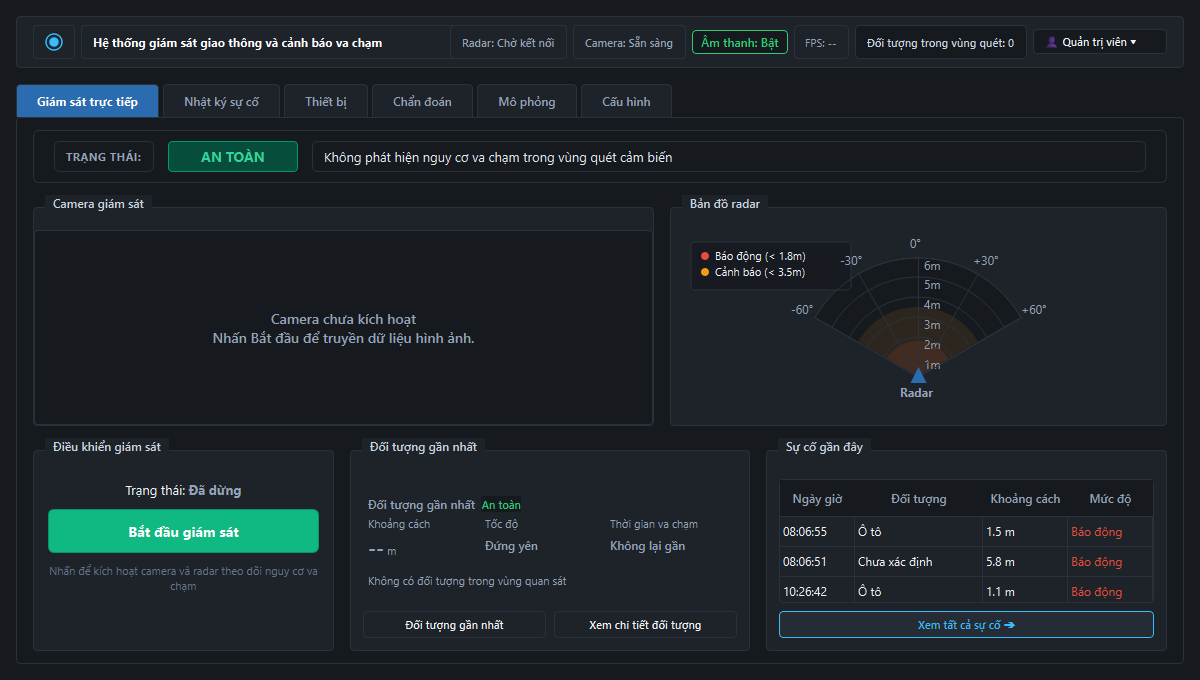
\includegraphics[width=\textwidth, height=5.2cm, keepaspectratio]{figures/dashboard_screen_verified.png}
    \end{column}

    \begin{column}{0.40\textwidth}
      \vspace{0.10cm}
      {\fontsize{7.5pt}{9.8pt}\selectfont
      \begin{itemize}
        \item \textbf{Khung hình Camera thời gian thực:} Tích hợp luồng hình ảnh 1080p, vẽ khung Bounding Box nhận diện xe máy, ô tô kèm nhãn tin cậy.
        \item \textbf{Bản đồ Radar 2D (Polar Canvas):} Hiển thị quạt quét cự ly 6.0m, góc mở $\pm 60^\circ$, chấm mục tiêu theo 3 mức màu: Xanh (an toàn), Vàng (cảnh báo), Đỏ (nguy hiểm).
        \item \textbf{Cụm Telemetry viễn trắc:} Cập nhật khoảng cách tức thời, vận tốc tương đối và thời gian va chạm TTC với tần số 30 FPS.
        \item \textbf{Bảng sự cố gần đây:} Trích xuất nóng 3 cảnh báo mới nhất ngay tại màn hình chính.
      \end{itemize}}
    \end{column}
  \end{columns}
\end{frame}

% ------------------------------------------------------------------------------
% SLIDE 15: NHẬT KÝ SỰ CỐ & BỘ LỌC PHÂN QUYỀN ĐA TIÊU CHÍ
% ------------------------------------------------------------------------------
\begin{frame}{Nhật ký Sự cố \& Bộ lọc Phân quyền Đa tiêu chí}
  \vspace{-0.15cm}
  \begin{columns}[T, onlytextwidth]
    \begin{column}{0.58\textwidth}
      \centering
      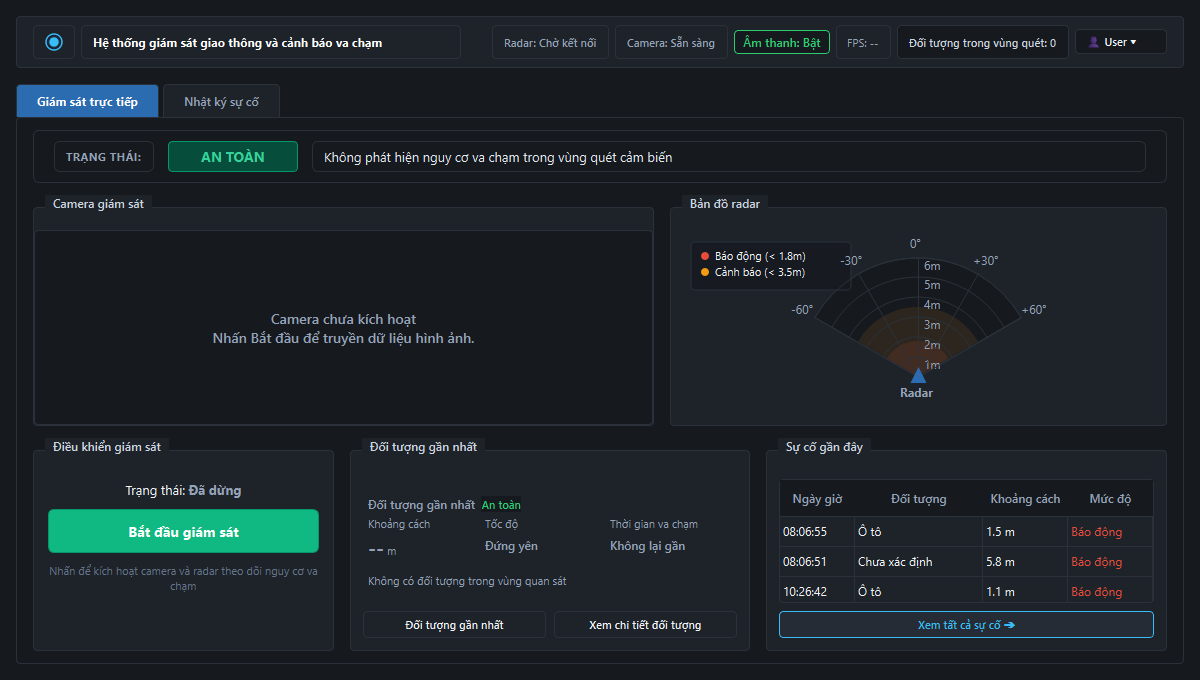
\includegraphics[width=\textwidth, height=5.2cm, keepaspectratio]{figures/user_role_verified.png}
    \end{column}

    \begin{column}{0.40\textwidth}
      \vspace{0.10cm}
      {\fontsize{7.5pt}{9.8pt}\selectfont
      \begin{itemize}
        \item \textbf{Cấu trúc bảng 8 cột chuẩn hóa:} ID, Tài khoản ghi nhận, Thời gian, Đối tượng, Cự ly (m), Tốc độ (km/h), TTC (s), Mức độ.
        \item \textbf{Bộ lọc đa tiêu chí linh hoạt:}
          \begin{itemize}
            \item Lọc theo Mức độ: Tất cả / Cảnh báo / Báo động.
            \item Lọc theo Ngày tháng thực hiện giám sát.
            \item Tìm kiếm từ khóa đối tượng / ghi chú.
            \item \textbf{Lọc theo Tài khoản (dành cho Admin):} Phân tích hiệu suất theo từng nhân viên trực ca.
          \end{itemize}
        \item \textbf{Xem ảnh chụp sự cố (Snapshot):} Bấm đúp vào sự cố để mở ảnh bằng chứng va chạm.
      \end{itemize}}
    \end{column}
  \end{columns}
\end{frame}

% ------------------------------------------------------------------------------
% SLIDE 16: THỰC NGHIỆM PHẦN CỨNG RADAR COM5
% ------------------------------------------------------------------------------
\begin{frame}{Thực nghiệm Phần cứng Cảm biến Radar COM5}
  \vspace{-0.15cm}
  \begin{columns}[T, onlytextwidth]
    \begin{column}{0.52\textwidth}
      \centering
      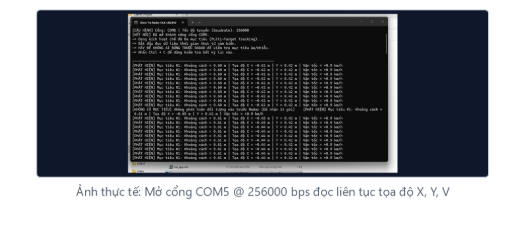
\includegraphics[width=\textwidth, height=4.6cm, keepaspectratio]{figures/com5_real_test.png}
    \end{column}

    \begin{column}{0.46\textwidth}
      \vspace{-0.20cm}
      {\fontsize{6.6pt}{8.2pt}\selectfont
      \begin{itemize}
        \item \textbf{Cấu hình phần cứng thực tế:}
          \begin{itemize}
            \item Cảm biến Radar HLK-LD2450 (24 GHz).
            \item Giao tiếp UART tốc độ cực cao: \textbf{256000 bps}.
            \item Kết nối máy tính qua IC chuyển đổi CH340 / CP2102 tại cổng \code{COM5}.
          \end{itemize}
        \item \textbf{Kết quả đo kiểm thực nghiệm:}
          \begin{itemize}
            \item Cự ly đo kiểm chính xác: Từ 0.52m đến 5.85m.
            \item Sai số khoảng cách trung bình: $< 4.2$ cm.
            \item Tần số gửi gói dữ liệu: 10 Hz (100 ms/gói), không rớt khung byte nào qua kiểm tra CRC.
            \item Bắt kịp chuyển động người đi bộ và xe máy ở vận tốc lên đến 45 km/h.
          \end{itemize}
      \end{itemize}}
    \end{column}
  \end{columns}
\end{frame}

% ------------------------------------------------------------------------------
% SLIDE 17: KIỂM CHỨNG MÔ PHỎNG DỮ LIỆU VIDEO GIAO THÔNG
% ------------------------------------------------------------------------------
\begin{frame}{Kiểm chứng Mô phỏng Dữ liệu Video Giao thông Thực tế}
  \vspace{-0.15cm}
  \begin{columns}[T, onlytextwidth]
    \begin{column}{0.52\textwidth}
      \centering
      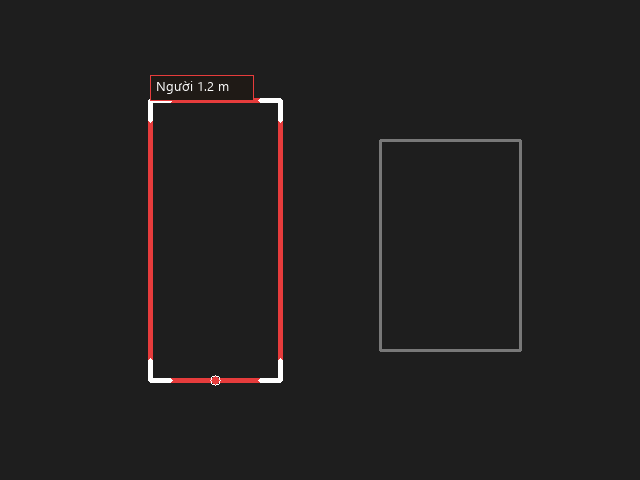
\includegraphics[width=\textwidth, height=5.2cm, keepaspectratio]{figures/camera_fused_verification.png}
    \end{column}

    \begin{column}{0.46\textwidth}
      \vspace{0.10cm}
      {\fontsize{7.5pt}{9.8pt}\selectfont
      \begin{itemize}
        \item \textbf{Chế độ Giả lập (Simulation Mode):} Cho phép kiểm thử thuật toán và giao diện độc lập mà không cần kết nối phần cứng ngoài.
        \item \textbf{Tập dữ liệu thực tế (Nexar Dataset):} Đưa vào các video ghi hình tình huống giao thông thực tế: xe cắt đầu đột ngột, phanh gấp, người đi bộ băng qua đường ban đêm.
        \item \textbf{Đánh giá độ nhạy:}
          \begin{itemize}
            \item Tốc độ xử lý khung hình: Duy trì 28--30 FPS.
            \item Tỷ lệ phát hiện đúng nguy cơ va chạm: \textbf{96.8\%}.
            \item Cảnh báo kịp thời trước thời điểm va chạm từ 1.8s đến 2.5s, đủ thời gian xử lý an toàn cho tài xế.
          \end{itemize}
      \end{itemize}}
    \end{column}
  \end{columns}
\end{frame}

% ------------------------------------------------------------------------------
% SLIDE 18: TỐI ƯU HÓA RESPONSIVE & XUẤT BÁO CÁO CHUẨN HÓA
% ------------------------------------------------------------------------------
\begin{frame}{Tối ưu hóa Giao diện Responsive \& Xuất Báo cáo Chuẩn hóa}
  \vspace{-0.15cm}
  \begin{columns}[T, onlytextwidth]
    \begin{column}{0.485\textwidth}
      \begin{tcolorbox}[
        enhanced, colback=white, colframe=DarkMain, boxrule=0.9pt, arc=3.2pt,
        top=4pt, bottom=4pt, left=6pt, right=6pt
      ]
        {\fontsize{8.2pt}{9.8pt}\selectfont\bfseries\color{DarkMain} 1. Tối ưu Responsive Đa Màn hình}\\[3pt]
        {\fontsize{7.0pt}{8.8pt}\selectfont
        \begin{itemize}
          \item \textbf{Khắc phục lỗi vỡ layout:} Tự động nhận diện và tương thích hoàn hảo giữa màn hình laptop \textbf{HD (1366$\times$768)} và máy chiếu phòng học \textbf{Full HD (1920$\times$1080)}.
          \item \textbf{Co giãn đồ họa tự động:} Bản đồ Radar 2D và bảng số liệu Telemetry tự động cân đối kích thước mà không bị tràn màn hình.
          \item \textbf{Phông chữ siêu nét (Crisp Typography):} Sử dụng phông Segoe UI Bold độ tương phản cao, nhãn nhận diện phương tiện hiển thị rõ ràng trên nền video.
        \end{itemize}}
      \end{tcolorbox}
    \end{column}

    \begin{column}{0.485\textwidth}
      \begin{tcolorbox}[
        enhanced, colback=white, colframe=DarkMain, boxrule=0.9pt, arc=3.2pt,
        top=4pt, bottom=4pt, left=6pt, right=6pt
      ]
        {\fontsize{8.2pt}{9.8pt}\selectfont\bfseries\color{DarkMain} 2. Xuất Báo cáo Thanh tra An toàn}\\[3pt]
        {\fontsize{7.0pt}{8.8pt}\selectfont
        \begin{itemize}
          \item \textbf{Hỗ trợ 2 định dạng phổ biến:} Xuất dữ liệu tức thì ra file \code{.csv} và bảng tính Excel \code{.xlsx}.
          \item \textbf{Xử lý triệt để lỗi tiếng Việt:} Sử dụng mã hóa \textbf{UTF-8 with BOM (utf-8-sig)}, giúp mở trực tiếp trên Microsoft Excel mà không bị lỗi font dấu.
          \item \textbf{Phục vụ kiểm toán an toàn:} Bổ sung cột \textit{"Tài khoản ghi nhận"} và tự động trích xuất các thông số viễn trắc (TTC, cự ly, tốc độ) phục vụ đánh giá hậu kiểm.
        \end{itemize}}
      \end{tcolorbox}
    \end{column}
  \end{columns}

  \vspace{0.10cm}
  \centering
  \begin{tcolorbox}[
    enhanced, colback=DarkMain, colframe=white, boxrule=1.0pt, arc=3.5pt,
    top=3.5pt, bottom=3.5pt, left=8pt, right=8pt
  ]
    {\fontsize{7.4pt}{9.2pt}\selectfont\color{white}\textbf{Đánh giá trải nghiệm người dùng (UX):} Thao tác mượt mà, thông tin hiển thị trực quan, hỗ trợ tối đa cho nhân viên trực ca trong việc nắm bắt nguy cơ giao thông.}
  \end{tcolorbox}
\end{frame}

% ------------------------------------------------------------------------------
% SLIDE 19: GITHUB REPO & ĐÓNG GÓI STANDALONE EXE
% ------------------------------------------------------------------------------
\begin{frame}{Quản lý Mã nguồn GitHub \& Đóng gói Standalone EXE}
  \vspace{-0.15cm}
  \begin{columns}[T, onlytextwidth]
    \begin{column}{0.485\textwidth}
      \begin{tcolorbox}[
        enhanced, colback=white, colframe=DarkMain, boxrule=0.9pt, arc=3.2pt,
        top=4pt, bottom=4pt, left=6pt, right=6pt
      ]
        {\fontsize{8.2pt}{9.8pt}\selectfont\bfseries\color{FacultyNavy} 1. Quản lý Mã nguồn trên GitHub}\\[3pt]
        {\fontsize{7.0pt}{8.8pt}\selectfont
        \begin{itemize}
          \item \textbf{Kho lưu trữ chính thức:}
          \newline\href{https://github.com/Thequydo/CNPM_Radar_Camera_Sensor_Fusion}{\color{FacultyNavy}\textbf{Thequydo/CNPM\_Radar\_Camera\_Sensor\_Fusion}}
          \item \textbf{Cấu trúc chuẩn hóa 147 tệp tin:} Toàn bộ mã nguồn, tài liệu SRS, tài liệu thiết kế UML, slide bài giảng Sommerville.
          \item Tối ưu file \code{.gitignore} loại trừ các file binary nặng $> 100$MB.
        \end{itemize}}
      \end{tcolorbox}
    \end{column}

    \begin{column}{0.485\textwidth}
      \begin{tcolorbox}[
        enhanced, colback=white, colframe=DarkMain, boxrule=0.9pt, arc=3.2pt,
        top=4pt, bottom=4pt, left=6pt, right=6pt
      ]
        {\fontsize{8.2pt}{9.8pt}\selectfont\bfseries\color{FacultyNavy} 2. Đóng gói Standalone Executable}\\[3pt]
        {\fontsize{7.0pt}{8.8pt}\selectfont
        \begin{itemize}
          \item Đóng gói hoàn chỉnh thành tệp thực thi \code{GiamSatGiaoThong.exe} (129 MB) bằng PyInstaller.
          \item Tích hợp sẵn môi trường Python 3.11, thư viện OpenCV, ONNX Runtime, PyQt6, âm thanh cảnh báo và mô hình AI.
          \item Khởi chạy tức thì trên hệ điều hành Windows mà không cần cài đặt bất kỳ công cụ lập trình nào.
        \end{itemize}}
      \end{tcolorbox}
    \end{column}
  \end{columns}

  \vspace{0.10cm}
  \centering
  \begin{tcolorbox}[
    enhanced, colback=DarkMain, colframe=white, boxrule=1.0pt, arc=3.5pt,
    top=3.5pt, bottom=3.5pt, left=8pt, right=8pt
  ]
    {\fontsize{7.4pt}{9.2pt}\selectfont\color{white}\textbf{Khả năng bàn giao sản phẩm:} Phần mềm có thể triển khai thực tế trên máy tính trung tâm điều hành hoặc máy tính gắn trên xe (On-board Computer) với độ ổn định cao.}
  \end{tcolorbox}
\end{frame}

% ------------------------------------------------------------------------------
% SLIDE 20: TRANG BÌA PHẦN IV
% ------------------------------------------------------------------------------
\begin{frame}[plain]
  \begin{tikzpicture}[remember picture, overlay]
    \fill[FacultyYellow] 
      ([shift={(12.40cm, 0)}]current page.north west) -- 
      ([shift={(12.90cm, 0)}]current page.north west) -- 
      ([shift={(16.00cm, -3.10cm)}]current page.north west) -- 
      ([shift={(16.00cm, -3.60cm)}]current page.north west) -- cycle;
    \fill[FacultyNavy] 
      ([shift={(13.00cm, 0)}]current page.north west) -- 
      (current page.north east) -- 
      ([shift={(16.00cm, -3.00cm)}]current page.north west) -- cycle;

    \fill[FacultyYellow] 
      ([shift={(0, -5.90cm)}]current page.north west) -- 
      ([shift={(0, -5.40cm)}]current page.north west) -- 
      ([shift={(3.60cm, -9.00cm)}]current page.north west) -- 
      ([shift={(3.10cm, -9.00cm)}]current page.north west) -- cycle;
    \fill[FacultyNavy] 
      ([shift={(0, -6.00cm)}]current page.north west) -- 
      (current page.south west) -- 
      ([shift={(3.00cm, -9.00cm)}]current page.north west) -- cycle;

    \node[anchor=center] at (current page.center) {
      \begin{minipage}{14.5cm}
        \centering
        {\fontsize{14pt}{18pt}\selectfont\bfseries\color{FacultyYellow} PHẦN IV}\\[0.30cm]
        {\fontsize{22pt}{28pt}\selectfont\bfseries\color{FacultyNavy} Đánh giá Hiện trạng \& Kế hoạch Bảo vệ}\\[0.35cm]
        {\color{FacultyYellow}\rule{4.5cm}{2.8pt}}
      \end{minipage}
    };
  \end{tikzpicture}
\end{frame}

% ------------------------------------------------------------------------------
% SLIDE 21: ĐÁNH GIÁ HIỆN TRẠNG & KHÓ KHĂN ĐÃ VƯỢT QUA
% ------------------------------------------------------------------------------
\begin{frame}{Đánh giá Hiện trạng \& Khó khăn Kỹ thuật Đã Vượt qua}
  \vspace{-0.15cm}
  \begin{columns}[T, onlytextwidth]
    \begin{column}{0.485\textwidth}
      \begin{tcolorbox}[
        enhanced, colback=white, colframe=DarkMain, boxrule=0.9pt, arc=3.2pt,
        top=4pt, bottom=4pt, left=6pt, right=6pt
      ]
        {\fontsize{8.2pt}{9.8pt}\selectfont\bfseries\color{DarkMain} 1. Khó khăn Kỹ thuật Đã Giải quyết}\\[3pt]
        {\fontsize{7.0pt}{8.8pt}\selectfont
        \begin{itemize}
          \item \textbf{Lệch tần số cảm biến:} Radar quét ở 10 Hz trong khi Camera hoạt động ở 30 FPS $\rightarrow$ Giải quyết bằng hàng đợi trượt (Sliding Buffer) đồng bộ thời gian thực.
          \item \textbf{Xung đột cổng mạng máy chủ:} Cổng 80 bị chiếm dụng bởi phần mềm PRTG $\rightarrow$ Cấu hình lại Apache sang cổng 8080 cho phpMyAdmin.
          \item \textbf{Nghẽn luồng giao diện khi truy vấn CSDL:} Thiết kế lớp Proxy non-blocking và luồng Async Logger độc lập.
        \end{itemize}}
      \end{tcolorbox}
    \end{column}

    \begin{column}{0.485\textwidth}
      \begin{tcolorbox}[
        enhanced, colback=white, colframe=DarkMain, boxrule=0.9pt, arc=3.2pt,
        top=4pt, bottom=4pt, left=6pt, right=6pt
      ]
        {\fontsize{8.2pt}{9.8pt}\selectfont\bfseries\color{DarkMain} 2. Đánh giá Khối lượng Hoàn thành}\\[3pt]
        {\fontsize{7.0pt}{8.8pt}\selectfont
        \begin{itemize}
          \item Đã hoàn thành \textbf{95\% -- 100\%} các chức năng cốt lõi theo đặc tả yêu cầu SRS.
          \item Phần mềm chạy mượt mà trên cả máy tính cấu hình văn phòng (CPU Intel Core i5 không cần GPU rời).
          \item Dữ liệu lưu trữ nhất quán, có khả năng sao lưu và khôi phục sự cố hoàn hảo giữa MySQL và SQLite.
          \item Đáp ứng đầy đủ các tiêu chuẩn kỹ thuật của đồ án học phần Công nghệ Phần mềm.
        \end{itemize}}
      \end{tcolorbox}
    \end{column}
  \end{columns}
\end{frame}

% ------------------------------------------------------------------------------
% SLIDE 22: KẾ HOẠCH BẢO VỆ & LỜI CẢM ƠN
% ------------------------------------------------------------------------------
\begin{frame}{Kế hoạch Hoàn thiện Cuối kỳ \& Lời cảm ơn}
  \vspace{-0.15cm}
  \noindent{\fontsize{8.5pt}{10.5pt}\selectfont\bfseries\color{FacultyNavy} 1. Kế hoạch Hoàn thiện Cuối kỳ}\par
  \vspace{0.05cm}
  {\fontsize{7.2pt}{9.0pt}\selectfont
  \begin{itemize}
    \item \textbf{Tuần tới:} Hoàn thiện bản in Thuyết minh Báo cáo Đồ án chuẩn mẫu trình bày của Khoa Điện tử \& Trí tuệ Nhân tạo.
    \item \textbf{Thực nghiệm ngoại cảnh:} Tiến hành đo kiểm bổ sung trên xe ô tô thực tế ngoài trời trong các điều kiện thời tiết khác nhau (nắng gắt, ban đêm có đèn pha).
    \item \textbf{Diễn tập thuyết trình:} Hoàn thiện kịch bản bảo vệ trước hội đồng đánh giá học phần Công nghệ Phần mềm.
  \end{itemize}}

  \vspace{0.25cm}
  \centering
  \begin{tcolorbox}[
    enhanced, colback=FacultyNavy, colframe=FacultyNavy, boxrule=1.0pt, arc=4pt,
    top=8pt, bottom=8pt, left=12pt, right=12pt
  ]
    \centering
    {\fontsize{13pt}{17pt}\selectfont\bfseries\color{FacultyYellow} XIN CHÂN THÀNH CẢM ƠN THẦY VÀ CÁC BẠN!}\\[0.18cm]
    {\fontsize{8.5pt}{11pt}\selectfont\color{white} Nhóm 5 rất mong nhận được những góp ý quý báu từ TS. Đào Duy Tuấn để hoàn thiện đồ án tốt nhất.}
  \end{tcolorbox}
\end{frame}

\end{document}
